\documentclass[11pt, a4paper, oneside]{article}

% URLs and hyperlinks ---------------------------------------
\usepackage{hyperref}
\hypersetup{
	colorlinks=true,
	linkcolor=blue,
	filecolor=magenta,      
	urlcolor=blue,
}
\usepackage[inline]{enumitem}
\usepackage{xurl}

% code snippet -------------------------------------------------------
\usepackage{minted}
% ---------------------------------------------------------------------

% page headers -------------------------------------------------
\usepackage{fancyhdr}
\fancypagestyle{plain}{\fancyhf{}\renewcommand{\headrulewidth}{0pt}}
\pagestyle{fancy}
\fancyhf{}
\fancyhead[L]{\nouppercase\leftmark}
\fancyhead[R]{\thepage}

% adjust a verrrrry big table -------------------------------
\usepackage{adjustbox}

% titlepage -------------------------------------------------
\usepackage{pdfpages}
\usepackage{svg}

% captions -------------------------------------------------
\usepackage[font=small,labelfont=bf]{caption}

% multiple figures ------------------------------------------
\usepackage{graphicx,subcaption}

% custom enumeration -----------------------------------------
\newcounter{itemadded}
\setcounter{itemadded}{0}
\newcommand{\addeditem}{%
	\addtocounter{enumi}{-1}%
	\stepcounter{itemadded}
	\let\LaTeXStandardLabelEnumi\labelenumi%
	\addtocounter{enumi}{1}
	\renewcommand{\labelenumi}{\arabic{enumi}\lr{R}.}%
	\item 
	\let\labelenumi\LaTeXStandardLabelEnumi%
}

\let\LaTeXStandardEnumerateBegin\enumerate
\let\LaTeXStandardEnumerateEnd\endenumerate

\renewenvironment{enumerate}{%
	\LaTeXStandardEnumerateBegin%
	\setcounter{itemadded}{0}
}{%
	\LaTeXStandardEnumerateEnd%
}

% tables -------------------------------------------------------
\usepackage{float}
\usepackage{multirow}
\renewcommand{\arraystretch}{1.23}

% Persian configuration ---------------------------------------
\usepackage{xepersian}
\settextfont{Yas}
\setdigitfont{Yas}
\setlatintextfont{Liberation Serif} % Use a dedicated Latin font for better spacing

% Line spacing adjustment -------------------------------------
\usepackage{setspace}
\linespread{1.5} % Adjust overall line spacing (1.0 for normal, 1.5 for increased)

\begin{document}
	
	\begin{titlepage}
		\centering
		\includesvg[width=3.8cm]{./layout/besm}\par
	
		\vspace{1cm}
    \includesvg[width=3.2cm]{./layout/logo}\par % Do not include the .svg extension
		
		\vspace{1mm}
		{\LARGE دانشگاه اصفهان}\par
		\vspace{1mm}
		{\Large دانشکده مهندسی کامپیوتر}\par
		
		\vspace{2cm}
		
		{\Large فاز چهارم پروژه در مبانی هوش و کاربردها}\par
		\vspace{1cm}
		{\Huge منطق درجه اول}\par
		
		
		\vspace{2cm}
		{\Large استاد درس: دکتر حسین کارشناس}\par
		\vspace{0.5cm}
		{\Large دستیار استاد: پوریا صامتی}
		
		\vspace{1cm}
		{\Large دانیال شفیعی}\par
		{\Large مهدی مهدیه}\par
		{\Large سید امیررضا نجفی}\par
		
		\vspace{1.5cm}
		
		% Bottom of the page
		{\large بهمن ۱۴۰۳\par}
	\end{titlepage}
	\tableofcontents
	\newpage

	\section{پرولوگ}
		برنامه از الگوریتم جستجوی هزینه یکنواخت برای پیداکردن کوتاه‌ترین مسیر استفاده می‌کند و مسیر را به یک لیست از اقدامات تبدیل می‌کند در کد پرولوگ عملیات زیر انجام می‌شود

		\subsection{
		بارگذاری و تجزیه نقشه 
		\lr{(Map Loading and Parsing)}
		}
		\begin{itemize}
			\item  
			\lr{read\_map(File)}
			: این بخش از کد مسئول خواندن فایل نقشه است. فایل نقشه شامل یک شبکه (گرید) است که موقعیت پرنده، خوک‌ها، سنگ‌ها و سلول‌های خالی را مشخص می‌کند. اگر در حین خواندن فایل خطایی رخ دهد، پیام خطا نمایش داده می‌شود.
			\item  \lr{read\_grid(Stream, Row)}
			:  این بخش هر خط از فایل را می‌خواند و آن را به‌عنوان یک‌رشته پردازش می‌کند. اگر خط به پایان فایل نرسیده باشد، خط پردازش می‌شود و شماره سطر افزایش می‌یابد.
			\item  \lr{process\_line(Line, Row, Col)}
			:  این بخش هر کاراکتر از خط را پردازش می‌کند. اگر کاراکتر معتبر باشد (مانند B برای پرنده، P برای خوک، R برای سنگ، و T برای سلول خالی)، موقعیت آن در شبکه ثبت می‌شود. اگر کاراکتر ناشناخته باشد، پیام خطا نمایش داده می‌شود.
		\end{itemize}
		\subsection{
پردازش سلول‌ها
\lr{ (Cell Processing)}
}
\begin {itemize}
\item {process\_cell} : این بخش کاراکترهای مختلف را پردازش می‌کند و موقعیت آن‌ها را در شبکه ثبت می‌کند:
\begin{itemize}
	\item B : موقعیت پرنده را تنظیم می‌کند.
	\item P : موقعیت خوک را اضافه می‌کند.
	\item R :  موقعیت سنگ را اضافه می‌کند.
	\item T : سلول خالی را نشان می‌دهد و هیچ عملی انجام نمی‌دهد.
	\item کاراکتر ناشناخته: پیام خطا نمایش داده می‌شود.
\end{itemize}
\end{itemize}
		

		
	\subsection{مدیریت وضعیت بازی
		\lr{ (State Management)}}
		\begin{itemize}
\item  : 
\lr{dynamic bird\_pos/2, dynamic pig\_pos/2, dynamic rock\_pos/2} :  این بخش از کد، موقعیت‌های پرنده، خوک‌ها و سنگ‌ها را به‌صورت پویا تعریف می‌کند تا در طول اجرای برنامه تغییر کنند.
\item \lr{set\_bird} :موقعیت پرنده را تنظیم می‌کند و موقعیت قبلی را پاک می‌کند.
\item \lr{ add\_pig} :  موقعیت خوک را اضافه می‌کند، اما فقط اگر قبلاً در آن موقعیت خوکی وجود نداشته باشد.
\item \lr{add\_rock} : موقعیت سنگ را اضافه می‌کند، اما فقط اگر قبلاً در آن موقعیت سنگی وجود نداشته باشد.
		\end{itemize}
	\subsection{تعریف حرکات 
		\lr{(Movement Definition)}}
	\begin{itemize}
		\item \lr{Move} : این بخش حرکات ممکن در گرید را تعریف می‌کند
		\begin{itemize}
			\item up: حرکت به بالا 
			\item Down : حرکت به پایین
			\item Left : حرکت به چپ 
			\item Right : حرکت به راست 
		\end{itemize}
		\item valid\_pos : این بخش بررسی می‌کند که آیا یک موقعیت در گرید معتبر است یا نه. یک موقعیت معتبر باید در گرید 8 در 8 باشد و روی سنگ قرار نگیرد.
	\end{itemize}

	
		\subsection{جستجوی مسیر بهینه (Pathfinding)}
		\begin{itemize}
			\item  find\_path : این بخش مسیر بهینه را برای رسیدن پرنده به تمام خوک‌ها پیدا می‌کند. ابتدا موقعیت پرنده و خوک‌ها را پیدا می‌کند، سپس مسیر بهینه را برای هر خوک محاسبه می‌کند.
			\item find\_optimal\_path : این بخش مسیر بهینه را برای رسیدن به هر خوک محاسبه می‌کند. از الگوریتم جستجوی هزینه یکنواخت 
			\lr{(Uniform Cost Search)}
			 استفاده می‌کند.
			\item Ucs : این بخش الگوریتم جستجوی هزینه یکنواخت را پیاده‌سازی می‌کند. این الگوریتم کوتاه‌ترین مسیر را از موقعیت فعلی پرنده به موقعیت خوک پیدا می‌کند.
			\item ucs\_search :این بخش جستجوی هزینه یکنواخت را انجام می‌دهد و مسیر بهینه را برمی‌گرداند.
		\end{itemize}

		\subsection{
		تبدیل مسیر به اقدامات 
		\lr{(Convert Path to Actions)}
	}
		
\begin{itemize}
	\item convert\_path\_to\_actions : این بخش مسیر پیدا شده را به یک لیست از اقدامات (حرکات) تبدیل می‌کند. هر حرکت با یک عدد مشخص می‌شود:
	\begin{itemize}
		\item  0 : حرکت به بالا.
		\item  1 : حرکت به پایین.
		\item  2 : حرکت به چپ.
		\item  3 : حرکت به راست.
	\end{itemize}
	\item get\_direction\_number : این بخش جهت حرکت بین دو سلول را مشخص می‌کند و آن را به یک عدد تبدیل می‌کند.
\end{itemize} 

		\section{پایتون}
		کد آی پایتون از کتابخانه‌های pyswip  و pygame استفاده می‌کند. در این گزارش، هر بخش از کد به طور کامل توضیح داده شده است.
		\subsection{
				بارگذاری و اجرای کد پرولوگ
				\lr{ (Prolog Integration)}
		}
\begin{itemize}
	\item \lr{prolog = Prolog()}
	:  یک شیء از کلاس Prolog  ایجاد می‌شود که امکان اجرای کد پرولوگ در پایتون را فراهم می‌کند.
	\item \lr{prolog.consult("x.pl")}
	: فایل پرولوگ x.pl که حاوی منطق بازی و الگوریتم‌های مسیریابی است، بارگذاری می‌شود.
	\item \lr{absolute\_path = str(Path(f'Env/templates/ {template}.txt').resolve()).replace('\\', '/')} : مسیر فایل نقشه (که موقعیت پرنده، خوک‌ها و سنگ‌ها را مشخص می‌کند) به‌صورت مطلق و با فرمت مناسب برای پرولوگ آماده می‌شود.
	\item \lr{list(prolog.query(f"read\_map(' {absolute\_path} ') "))} : نقشه از فایل خوانده می‌شود و موقعیت‌ها در پرولوگ ثبت می‌شوند.
	دریافت موقعیت‌ها از پرولوگ
	\lr{ (Querying Prolog for Positions)}
	\item \lr{print(list(prolog.query('pig\_pos(X, Y)')))} : موقعیت تمام خوک‌ها از پرولوگ دریافت و چاپ می‌شود.
	\item \lr{bird\_pos = env.get\_bird\_position()} : موقعیت پرنده از محیط بازی دریافت می‌شود.
	\item \lr{print(list(prolog.query('bird\_pos(X, Y)')))}: موقعیت پرنده از پرولوگ دریافت و چاپ می‌شود.
	\item \lr{print(list(prolog.query('findall((PX, PY), pig\_pos(PX, PY), Pigs)')))} : موقعیت تمام خوک‌ها از پرولوگ دریافت و چاپ می‌شود.
\end{itemize}
		
		\subsection{
				یافتن مسیر بهینه 
				\lr{(Finding the Optimal Path)}
		}
	
\begin{itemize}
	\item \lr{solutions = list(prolog.query(f"find\_path(Actions)"))} : مسیر بهینه برای رسیدن پرنده به تمام خوک‌ها از پرولوگ دریافت می‌شود.
	\item \lr{lengths = [len(d ['Actions']) for d in solutions]} : طول هر مسیر محاسبه می‌شود.
	\item \lr{min\_length = min(lengths)}: کوتاه‌ترین طول مسیر پیدا می‌شود.
	\item \lr{optimal\_solutions = [d for d in solutions if len(d ['Actions']) == min\_length]} : مسیرهای بهینه (با کمترین طول) انتخاب می‌شوند.
	\item \lr{actions = optimal\_solutions [0] ['Actions']} : اولین مسیر بهینه انتخاب می‌شود.
	\item print(actions) : اقدامات (حرکات) مربوط به مسیر بهینه چاپ می‌شوند.
	\item print(lengths) : طول‌های تمام مسیرها چاپ می‌شوند.
	\item print(solutions) : تمام مسیرهای پیدا شده چاپ می‌شوند.
\end{itemize}		
\section{اجرا روی نقشه‌ها}
\begin{figure}
	\centering
	\begin{subfigure}{0.5\textwidth}
		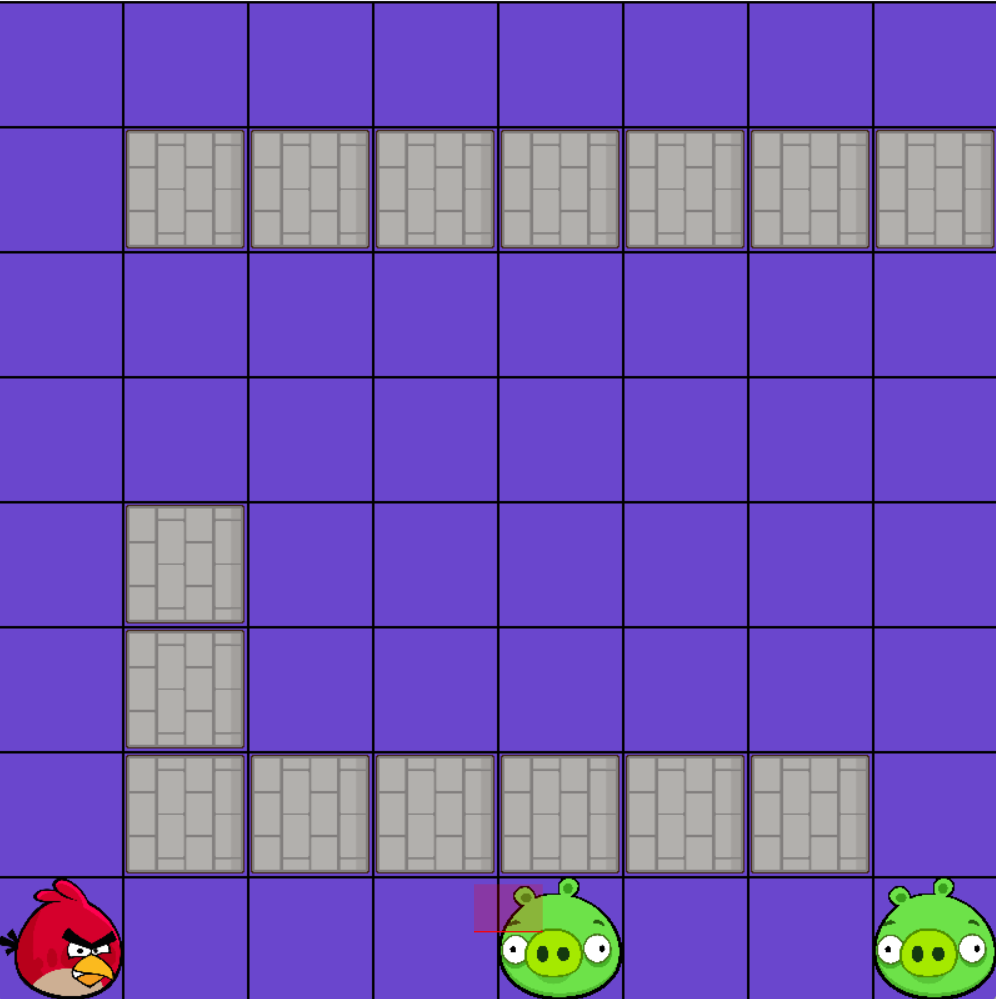
\includegraphics[width=\textwidth]{./images/simple}
		\caption{اجرا روی محیط ساده}
		\label{fig:simplemap}
	\end{subfigure}
\hfill
	\begin{subfigure}{0.5\textwidth}
		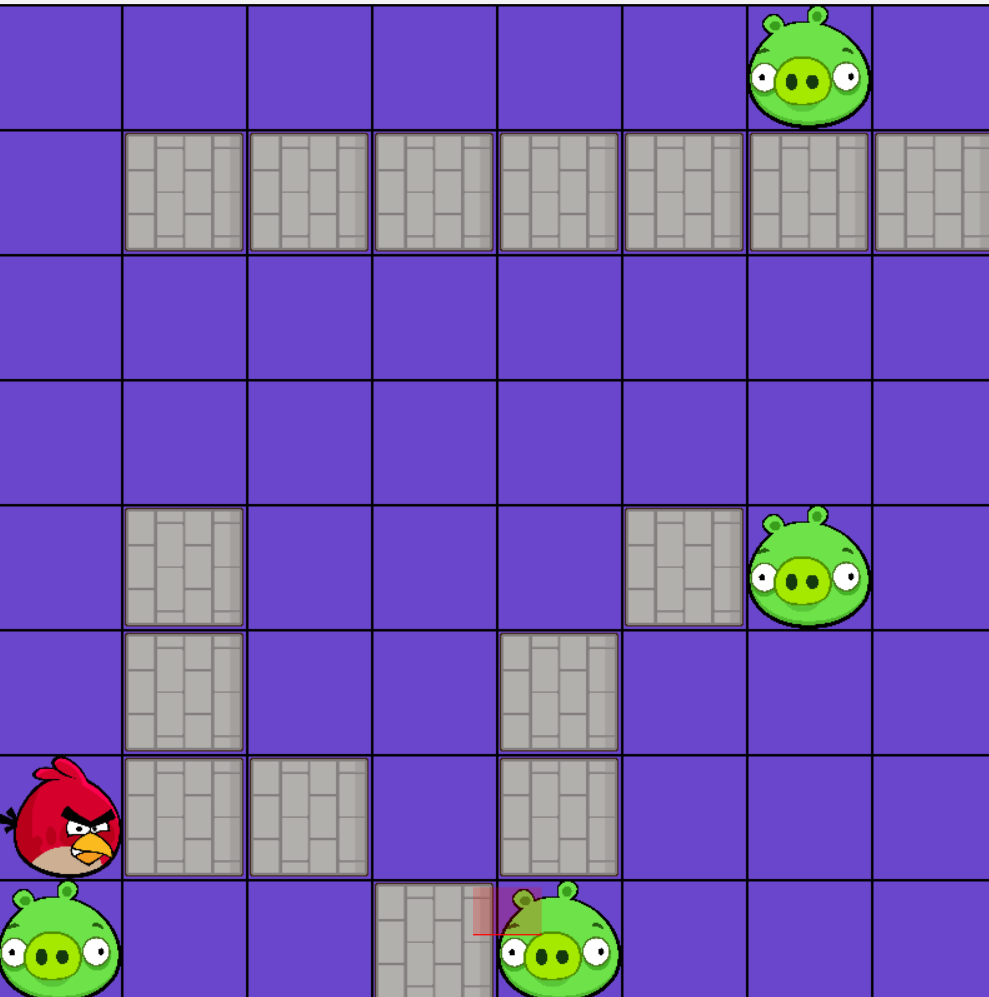
\includegraphics[width=\textwidth]{./images/map1}
		\caption{اجرا روی نقشه‌ی تولید شده ۱}
		\label{fig:map1}
	\end{subfigure}
\medskip
	\begin{subfigure}{0.5\textwidth}
		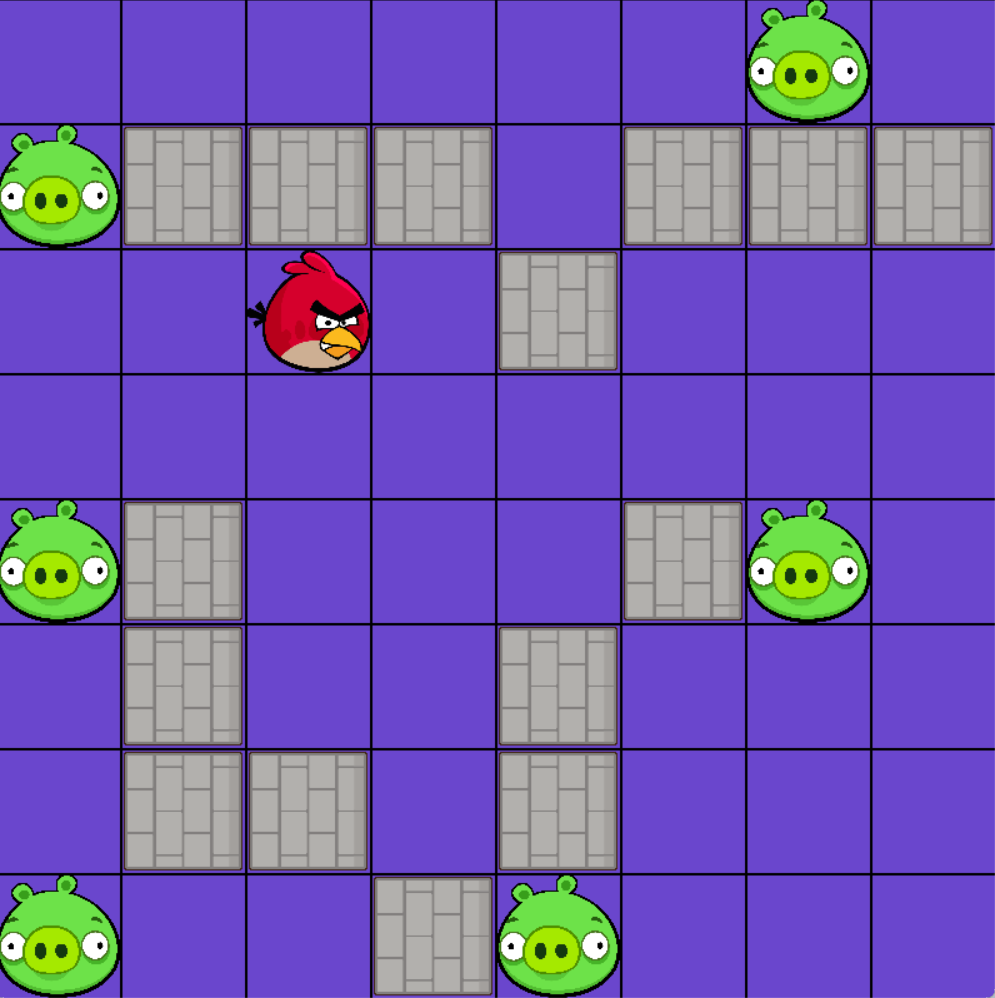
\includegraphics[width=\textwidth]{./images/map2}
		\caption{اجرا روی نقشه‌ی تولید شده‌ی ۲}
		\label{fig:map2}
	\end{subfigure}
	\caption{اجرا روی محیط‌ها}
	\label{Grids}
\end{figure}
\end{document}